\documentclass[twoside]{book}

% Packages required by doxygen
\usepackage{fixltx2e}
\usepackage{calc}
\usepackage{doxygen}
\usepackage[export]{adjustbox} % also loads graphicx
\usepackage{graphicx}
\usepackage[utf8]{inputenc}
\usepackage{makeidx}
\usepackage{multicol}
\usepackage{multirow}
\PassOptionsToPackage{warn}{textcomp}
\usepackage{textcomp}
\usepackage[nointegrals]{wasysym}
\usepackage[table]{xcolor}

% Font selection
\usepackage[T1]{fontenc}
\usepackage[scaled=.90]{helvet}
\usepackage{courier}
\usepackage{amssymb}
\usepackage{sectsty}
\renewcommand{\familydefault}{\sfdefault}
\allsectionsfont{%
  \fontseries{bc}\selectfont%
  \color{darkgray}%
}
\renewcommand{\DoxyLabelFont}{%
  \fontseries{bc}\selectfont%
  \color{darkgray}%
}
\newcommand{\+}{\discretionary{\mbox{\scriptsize$\hookleftarrow$}}{}{}}

% Page & text layout
\usepackage{geometry}
\geometry{%
  a4paper,%
  top=2.5cm,%
  bottom=2.5cm,%
  left=2.5cm,%
  right=2.5cm%
}
\tolerance=750
\hfuzz=15pt
\hbadness=750
\setlength{\emergencystretch}{15pt}
\setlength{\parindent}{0cm}
\setlength{\parskip}{3ex plus 2ex minus 2ex}
\makeatletter
\renewcommand{\paragraph}{%
  \@startsection{paragraph}{4}{0ex}{-1.0ex}{1.0ex}{%
    \normalfont\normalsize\bfseries\SS@parafont%
  }%
}
\renewcommand{\subparagraph}{%
  \@startsection{subparagraph}{5}{0ex}{-1.0ex}{1.0ex}{%
    \normalfont\normalsize\bfseries\SS@subparafont%
  }%
}
\makeatother

% Headers & footers
\usepackage{fancyhdr}
\pagestyle{fancyplain}
\fancyhead[LE]{\fancyplain{}{\bfseries\thepage}}
\fancyhead[CE]{\fancyplain{}{}}
\fancyhead[RE]{\fancyplain{}{\bfseries\leftmark}}
\fancyhead[LO]{\fancyplain{}{\bfseries\rightmark}}
\fancyhead[CO]{\fancyplain{}{}}
\fancyhead[RO]{\fancyplain{}{\bfseries\thepage}}
\fancyfoot[LE]{\fancyplain{}{}}
\fancyfoot[CE]{\fancyplain{}{}}
\fancyfoot[RE]{\fancyplain{}{\bfseries\scriptsize Generated by Doxygen }}
\fancyfoot[LO]{\fancyplain{}{\bfseries\scriptsize Generated by Doxygen }}
\fancyfoot[CO]{\fancyplain{}{}}
\fancyfoot[RO]{\fancyplain{}{}}
\renewcommand{\footrulewidth}{0.4pt}
\renewcommand{\chaptermark}[1]{%
  \markboth{#1}{}%
}
\renewcommand{\sectionmark}[1]{%
  \markright{\thesection\ #1}%
}

% Indices & bibliography
\usepackage{natbib}
\usepackage[titles]{tocloft}
\setcounter{tocdepth}{3}
\setcounter{secnumdepth}{5}
\makeindex

% Hyperlinks (required, but should be loaded last)
\usepackage{ifpdf}
\ifpdf
  \usepackage[pdftex,pagebackref=true]{hyperref}
\else
  \usepackage[ps2pdf,pagebackref=true]{hyperref}
\fi
\hypersetup{%
  colorlinks=true,%
  linkcolor=blue,%
  citecolor=blue,%
  unicode%
}

% Custom commands
\newcommand{\clearemptydoublepage}{%
  \newpage{\pagestyle{empty}\cleardoublepage}%
}

\usepackage{caption}
\captionsetup{labelsep=space,justification=centering,font={bf},singlelinecheck=off,skip=4pt,position=top}

%===== C O N T E N T S =====

\begin{document}

% Titlepage & ToC
\hypersetup{pageanchor=false,
             bookmarksnumbered=true,
             pdfencoding=unicode
            }
\pagenumbering{alph}
\begin{titlepage}
\vspace*{7cm}
\begin{center}%
{\Large D\+S\+SD Doxy }\\
\vspace*{1cm}
{\large Generated by Doxygen 1.8.13}\\
\end{center}
\end{titlepage}
\clearemptydoublepage
\pagenumbering{roman}
\tableofcontents
\clearemptydoublepage
\pagenumbering{arabic}
\hypersetup{pageanchor=true}

%--- Begin generated contents ---
\chapter{Namespace Index}
\section{Namespace List}
Here is a list of all documented namespaces with brief descriptions\+:\begin{DoxyCompactList}
\item\contentsline{section}{\hyperlink{namespace_ui}{Ui} \\*\hyperlink{class_main_window}{Main\+Window} This is the baseline UI }{\pageref{namespace_ui}}{}
\end{DoxyCompactList}

\chapter{Hierarchical Index}
\section{Class Hierarchy}
This inheritance list is sorted roughly, but not completely, alphabetically\+:\begin{DoxyCompactList}
\item \contentsline{section}{D\+B\+Manager}{\pageref{class_d_b_manager}}{}
\item \contentsline{section}{Distance}{\pageref{class_distance}}{}
\item \contentsline{section}{Menu\+Item}{\pageref{class_menu_item}}{}
\item Q\+Dialog\begin{DoxyCompactList}
\item \contentsline{section}{add\+Menu\+Item}{\pageref{classadd_menu_item}}{}
\item \contentsline{section}{change\+Price}{\pageref{classchange_price}}{}
\end{DoxyCompactList}
\item Q\+Main\+Window\begin{DoxyCompactList}
\item \contentsline{section}{Admin}{\pageref{class_admin}}{}
\item \contentsline{section}{Main\+Window}{\pageref{class_main_window}}{}
\end{DoxyCompactList}
\item Q\+Widget\begin{DoxyCompactList}
\item \contentsline{section}{Trip\+Screen}{\pageref{class_trip_screen}}{}
\end{DoxyCompactList}
\item \contentsline{section}{Restaurant}{\pageref{class_restaurant}}{}
\end{DoxyCompactList}

\chapter{Class Index}
\section{Class List}
Here are the classes, structs, unions and interfaces with brief descriptions\+:\begin{DoxyCompactList}
\item\contentsline{section}{\hyperlink{classadd_menu_item}{add\+Menu\+Item} }{\pageref{classadd_menu_item}}{}
\item\contentsline{section}{\hyperlink{class_admin}{Admin} \\*The \hyperlink{class_admin}{Admin} class }{\pageref{class_admin}}{}
\item\contentsline{section}{\hyperlink{classchange_price}{change\+Price} }{\pageref{classchange_price}}{}
\item\contentsline{section}{\hyperlink{class_d_b_manager}{D\+B\+Manager} \\*The \hyperlink{class_d_b_manager}{D\+B\+Manager} class }{\pageref{class_d_b_manager}}{}
\item\contentsline{section}{\hyperlink{class_distance}{Distance} \\*The \hyperlink{class_distance}{Distance} class }{\pageref{class_distance}}{}
\item\contentsline{section}{\hyperlink{class_main_window}{Main\+Window} }{\pageref{class_main_window}}{}
\item\contentsline{section}{\hyperlink{class_menu_item}{Menu\+Item} \\*The \hyperlink{class_menu_item}{Menu\+Item} class }{\pageref{class_menu_item}}{}
\item\contentsline{section}{\hyperlink{class_restaurant}{Restaurant} \\*The \hyperlink{class_restaurant}{Restaurant} class }{\pageref{class_restaurant}}{}
\item\contentsline{section}{\hyperlink{class_trip_screen}{Trip\+Screen} }{\pageref{class_trip_screen}}{}
\end{DoxyCompactList}

\chapter{Namespace Documentation}
\hypertarget{namespace_ui}{}\section{Ui Namespace Reference}
\label{namespace_ui}\index{Ui@{Ui}}


\hyperlink{class_main_window}{Main\+Window} This is the baseline UI.  




\subsection{Detailed Description}
\hyperlink{class_main_window}{Main\+Window} This is the baseline UI. 
\chapter{Class Documentation}
\hypertarget{classadd_menu_item}{}\section{add\+Menu\+Item Class Reference}
\label{classadd_menu_item}\index{add\+Menu\+Item@{add\+Menu\+Item}}
Inheritance diagram for add\+Menu\+Item\+:\begin{figure}[H]
\begin{center}
\leavevmode
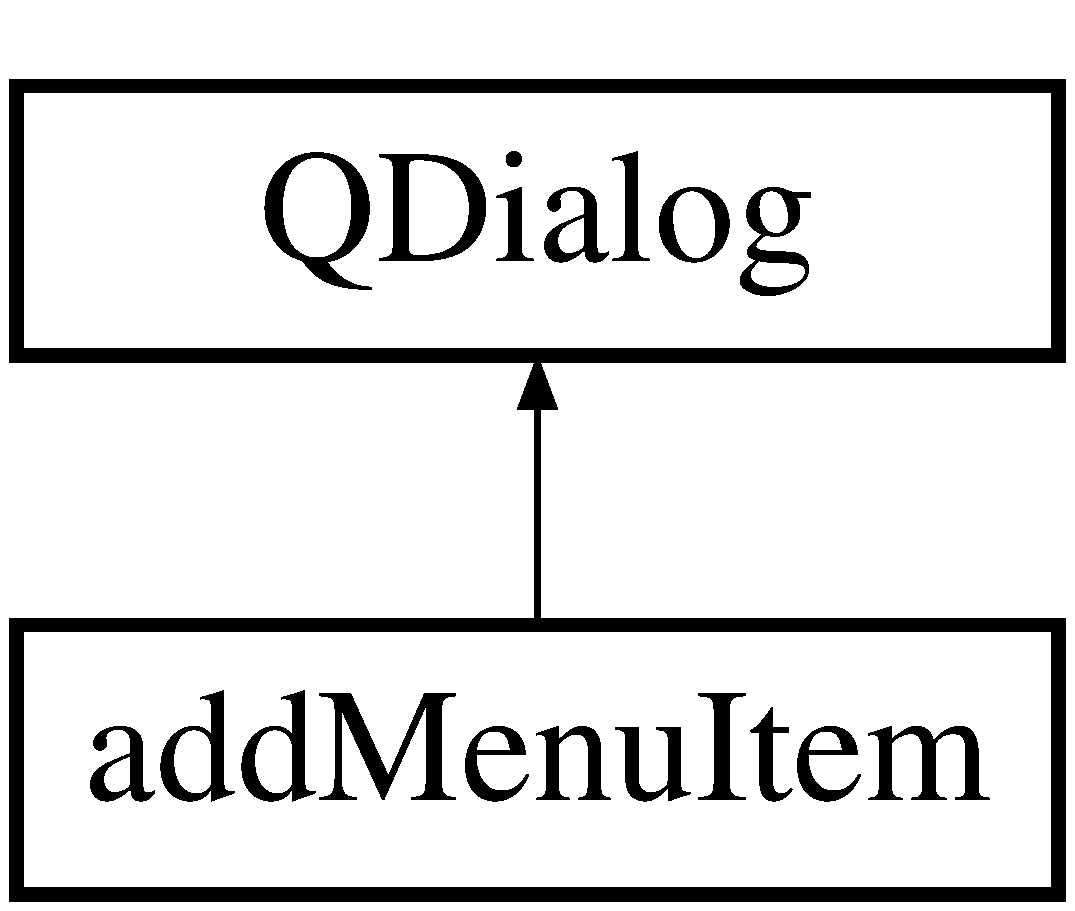
\includegraphics[height=2.000000cm]{classadd_menu_item}
\end{center}
\end{figure}
\subsection*{Public Member Functions}
\begin{DoxyCompactItemize}
\item 
\mbox{\Hypertarget{classadd_menu_item_a516e0cb12135a23a4378d1f0c69b3166}\label{classadd_menu_item_a516e0cb12135a23a4378d1f0c69b3166}} 
{\bfseries add\+Menu\+Item} (Q\+Widget $\ast$parent=0)
\end{DoxyCompactItemize}


The documentation for this class was generated from the following files\+:\begin{DoxyCompactItemize}
\item 
addmenuitem.\+h\item 
addmenuitem.\+cpp\end{DoxyCompactItemize}

\hypertarget{class_admin}{}\section{Admin Class Reference}
\label{class_admin}\index{Admin@{Admin}}


The \hyperlink{class_admin}{Admin} class.  




{\ttfamily \#include $<$admin.\+h$>$}

Inheritance diagram for Admin\+:\begin{figure}[H]
\begin{center}
\leavevmode
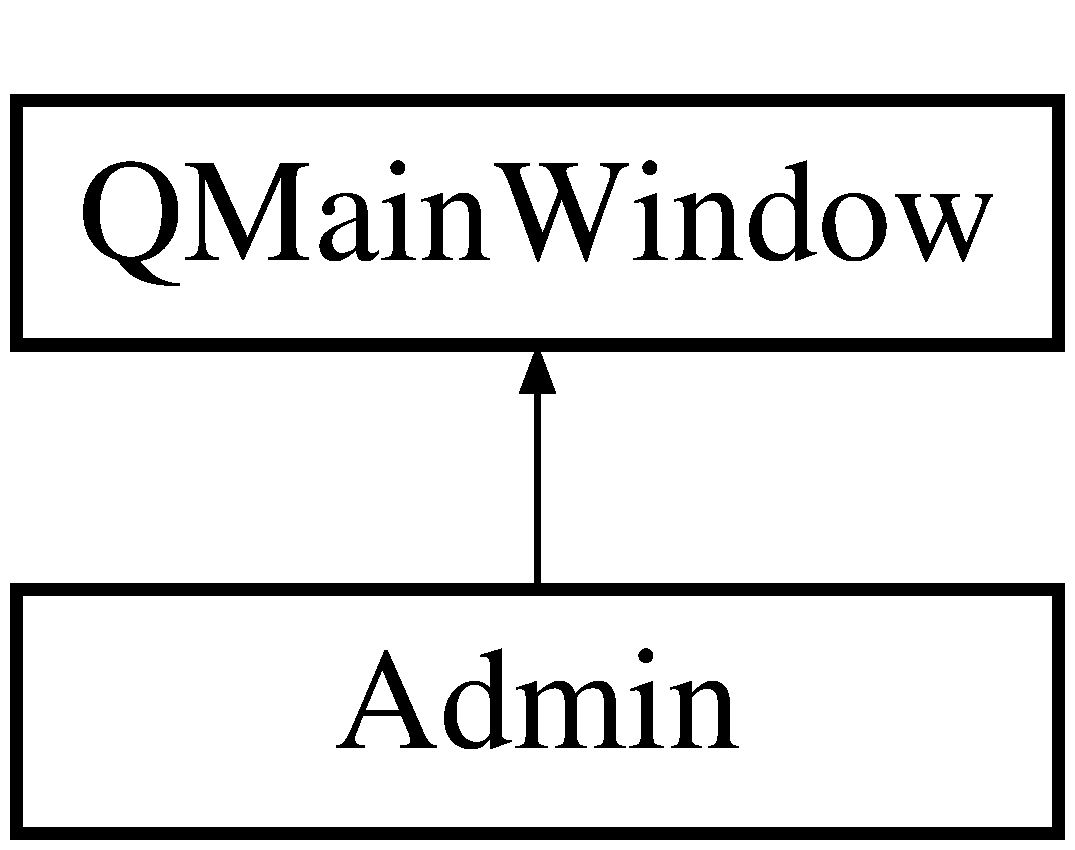
\includegraphics[height=2.000000cm]{class_admin}
\end{center}
\end{figure}
\subsection*{Public Member Functions}
\begin{DoxyCompactItemize}
\item 
\mbox{\Hypertarget{class_admin_a5e67a0ecb1fc8cd09c0f340b03be4016}\label{class_admin_a5e67a0ecb1fc8cd09c0f340b03be4016}} 
{\bfseries Admin} (Q\+Widget $\ast$parent=0)
\end{DoxyCompactItemize}


\subsection{Detailed Description}
The \hyperlink{class_admin}{Admin} class. 

The documentation for this class was generated from the following files\+:\begin{DoxyCompactItemize}
\item 
admin.\+h\item 
admin.\+cpp\end{DoxyCompactItemize}

\hypertarget{classchange_price}{}\section{change\+Price Class Reference}
\label{classchange_price}\index{change\+Price@{change\+Price}}
Inheritance diagram for change\+Price\+:\begin{figure}[H]
\begin{center}
\leavevmode
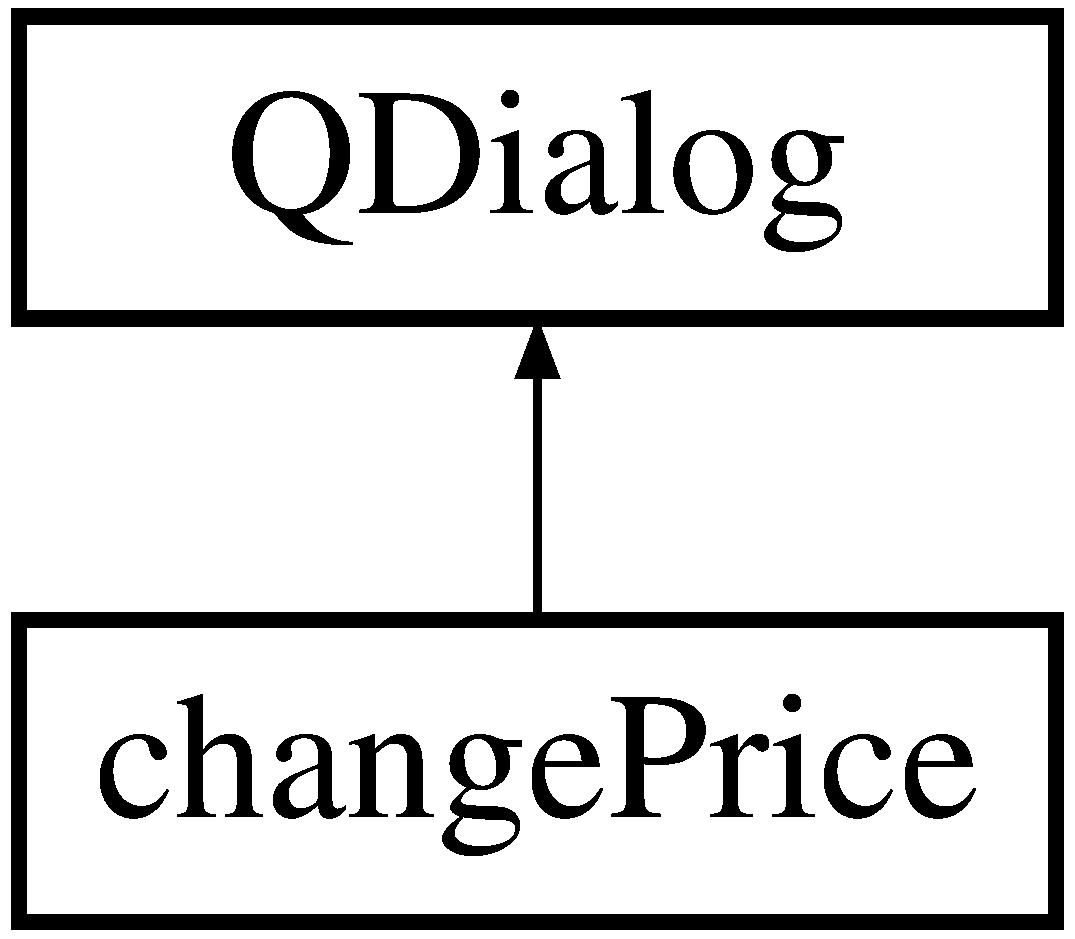
\includegraphics[height=2.000000cm]{classchange_price}
\end{center}
\end{figure}
\subsection*{Public Member Functions}
\begin{DoxyCompactItemize}
\item 
\mbox{\Hypertarget{classchange_price_a7bd9c2db0a96fc215d5d1ff7bbe404db}\label{classchange_price_a7bd9c2db0a96fc215d5d1ff7bbe404db}} 
{\bfseries change\+Price} (Q\+Widget $\ast$parent=0)
\end{DoxyCompactItemize}


The documentation for this class was generated from the following files\+:\begin{DoxyCompactItemize}
\item 
changeprice.\+h\item 
changeprice.\+cpp\end{DoxyCompactItemize}

\hypertarget{class_d_b_manager}{}\section{D\+B\+Manager Class Reference}
\label{class_d_b_manager}\index{D\+B\+Manager@{D\+B\+Manager}}


The \hyperlink{class_d_b_manager}{D\+B\+Manager} class.  




{\ttfamily \#include $<$dbmanager.\+h$>$}

\subsection*{Public Member Functions}
\begin{DoxyCompactItemize}
\item 
void \hyperlink{class_d_b_manager_a2d29cb558fdbf54d17b180088bd8651e}{upload\+File\+To\+Database} (const Q\+String \&file\+Path)
\begin{DoxyCompactList}\small\item\em upload\+File\+To\+Database \end{DoxyCompactList}\item 
void \hyperlink{class_d_b_manager_a914d5a2d66ddff2b0a39c545966540e9}{database\+To\+Restaurants} ()
\begin{DoxyCompactList}\small\item\em database\+To\+Restaurants \end{DoxyCompactList}\item 
std\+::vector$<$ \hyperlink{class_restaurant}{Restaurant} $>$ \hyperlink{class_d_b_manager_ab726a1be7b797085723623f5497946e6}{get\+Restaurants} ()
\begin{DoxyCompactList}\small\item\em get\+Restaurants \end{DoxyCompactList}\item 
\mbox{\Hypertarget{class_d_b_manager_aa90cd2919d5e288ec5656e4d0abfdbe4}\label{class_d_b_manager_aa90cd2919d5e288ec5656e4d0abfdbe4}} 
void {\bfseries test\+DB} ()
\item 
void \hyperlink{class_d_b_manager_ac2f9bedac3778197de1301775ef8d42f}{Delete\+From\+Db} (Q\+String name)
\begin{DoxyCompactList}\small\item\em Delete\+From\+Db. \end{DoxyCompactList}\end{DoxyCompactItemize}
\subsection*{Static Public Member Functions}
\begin{DoxyCompactItemize}
\item 
\mbox{\Hypertarget{class_d_b_manager_ad386a91c5c54a9e34e793b35ec0957c8}\label{class_d_b_manager_ad386a91c5c54a9e34e793b35ec0957c8}} 
static \hyperlink{class_d_b_manager}{D\+B\+Manager} $\ast$ {\bfseries get\+Instance} ()
\end{DoxyCompactItemize}


\subsection{Detailed Description}
The \hyperlink{class_d_b_manager}{D\+B\+Manager} class. 

\begin{DoxyAuthor}{Author}
Sean O\textquotesingle{}Hearn
\end{DoxyAuthor}
Manages the database by allowing the manipulation of data within the database. Uses singleton desgin pattern. 

\subsection{Member Function Documentation}
\mbox{\Hypertarget{class_d_b_manager_a914d5a2d66ddff2b0a39c545966540e9}\label{class_d_b_manager_a914d5a2d66ddff2b0a39c545966540e9}} 
\index{D\+B\+Manager@{D\+B\+Manager}!database\+To\+Restaurants@{database\+To\+Restaurants}}
\index{database\+To\+Restaurants@{database\+To\+Restaurants}!D\+B\+Manager@{D\+B\+Manager}}
\subsubsection{\texorpdfstring{database\+To\+Restaurants()}{databaseToRestaurants()}}
{\footnotesize\ttfamily void D\+B\+Manager\+::database\+To\+Restaurants (\begin{DoxyParamCaption}{ }\end{DoxyParamCaption})}



database\+To\+Restaurants 

Uses the database to populate our vector filled with \hyperlink{class_restaurant}{Restaurant} objects \mbox{\Hypertarget{class_d_b_manager_ac2f9bedac3778197de1301775ef8d42f}\label{class_d_b_manager_ac2f9bedac3778197de1301775ef8d42f}} 
\index{D\+B\+Manager@{D\+B\+Manager}!Delete\+From\+Db@{Delete\+From\+Db}}
\index{Delete\+From\+Db@{Delete\+From\+Db}!D\+B\+Manager@{D\+B\+Manager}}
\subsubsection{\texorpdfstring{Delete\+From\+Db()}{DeleteFromDb()}}
{\footnotesize\ttfamily void D\+B\+Manager\+::\+Delete\+From\+Db (\begin{DoxyParamCaption}\item[{Q\+String}]{name }\end{DoxyParamCaption})}



Delete\+From\+Db. 


\begin{DoxyParams}{Parameters}
{\em name} & \\
\hline
\end{DoxyParams}
\mbox{\Hypertarget{class_d_b_manager_ab726a1be7b797085723623f5497946e6}\label{class_d_b_manager_ab726a1be7b797085723623f5497946e6}} 
\index{D\+B\+Manager@{D\+B\+Manager}!get\+Restaurants@{get\+Restaurants}}
\index{get\+Restaurants@{get\+Restaurants}!D\+B\+Manager@{D\+B\+Manager}}
\subsubsection{\texorpdfstring{get\+Restaurants()}{getRestaurants()}}
{\footnotesize\ttfamily std\+::vector$<$ \hyperlink{class_restaurant}{Restaurant} $>$ D\+B\+Manager\+::get\+Restaurants (\begin{DoxyParamCaption}{ }\end{DoxyParamCaption})}



get\+Restaurants 

\begin{DoxyReturn}{Returns}
restaurants 
\end{DoxyReturn}
\mbox{\Hypertarget{class_d_b_manager_a2d29cb558fdbf54d17b180088bd8651e}\label{class_d_b_manager_a2d29cb558fdbf54d17b180088bd8651e}} 
\index{D\+B\+Manager@{D\+B\+Manager}!upload\+File\+To\+Database@{upload\+File\+To\+Database}}
\index{upload\+File\+To\+Database@{upload\+File\+To\+Database}!D\+B\+Manager@{D\+B\+Manager}}
\subsubsection{\texorpdfstring{upload\+File\+To\+Database()}{uploadFileToDatabase()}}
{\footnotesize\ttfamily void D\+B\+Manager\+::upload\+File\+To\+Database (\begin{DoxyParamCaption}\item[{const Q\+String \&}]{file\+Path }\end{DoxyParamCaption})}



upload\+File\+To\+Database 


\begin{DoxyParams}{Parameters}
{\em file\+Path} & \\
\hline
\end{DoxyParams}


The documentation for this class was generated from the following files\+:\begin{DoxyCompactItemize}
\item 
dbmanager.\+h\item 
dbmanager.\+cpp\end{DoxyCompactItemize}

\hypertarget{class_distance}{}\section{Distance Class Reference}
\label{class_distance}\index{Distance@{Distance}}


The \hyperlink{class_distance}{Distance} class.  




{\ttfamily \#include $<$distance.\+h$>$}

\subsection*{Public Member Functions}
\begin{DoxyCompactItemize}
\item 
\mbox{\Hypertarget{class_distance_a32421795b03aa6284476000229aa1c17}\label{class_distance_a32421795b03aa6284476000229aa1c17}} 
{\bfseries Distance} (double distance\+In\+Miles, int restaurant\+I\+D\+From, int restaurant\+I\+D\+To)
\item 
void \hyperlink{class_distance_a2bbd9bef5a6f0692aa1b4d8b5ce9344f}{set\+Distance\+In\+Miles} (double distance\+In\+Miles)
\begin{DoxyCompactList}\small\item\em set\+Distance\+In\+Miles \end{DoxyCompactList}\item 
void \hyperlink{class_distance_ae91858d0705925be8f96d586844697ec}{set\+Restaurant\+I\+D\+From} (int restaurant\+I\+D\+From)
\begin{DoxyCompactList}\small\item\em set\+Restaurant\+I\+D\+From \end{DoxyCompactList}\item 
void \hyperlink{class_distance_a3fc24cd557605c2731ed9f379da3bb94}{set\+Restaurant\+I\+D\+To} (int restaurant\+I\+D\+To)
\begin{DoxyCompactList}\small\item\em set\+Restaurant\+I\+D\+To \end{DoxyCompactList}\item 
double \hyperlink{class_distance_acc0170b8899fed2a86e4487e12b1ebe9}{get\+Distance\+In\+Miles} ()
\begin{DoxyCompactList}\small\item\em get\+Distance\+In\+Miles \end{DoxyCompactList}\item 
int \hyperlink{class_distance_a6aad4761255f0a1dafafab7e98283a81}{get\+Restaurant\+I\+D\+From} ()
\begin{DoxyCompactList}\small\item\em get\+Restaurant\+I\+D\+From \end{DoxyCompactList}\item 
int \hyperlink{class_distance_ad523bb34afe88d178a1cb494220244bb}{get\+Restaurant\+I\+D\+To} ()
\begin{DoxyCompactList}\small\item\em get\+Restaurant\+I\+D\+To \end{DoxyCompactList}\end{DoxyCompactItemize}


\subsection{Detailed Description}
The \hyperlink{class_distance}{Distance} class. 

\begin{DoxyAuthor}{Author}
Sean O\textquotesingle{}Hearn Container for distances between restaurants 
\end{DoxyAuthor}


\subsection{Member Function Documentation}
\mbox{\Hypertarget{class_distance_acc0170b8899fed2a86e4487e12b1ebe9}\label{class_distance_acc0170b8899fed2a86e4487e12b1ebe9}} 
\index{Distance@{Distance}!get\+Distance\+In\+Miles@{get\+Distance\+In\+Miles}}
\index{get\+Distance\+In\+Miles@{get\+Distance\+In\+Miles}!Distance@{Distance}}
\subsubsection{\texorpdfstring{get\+Distance\+In\+Miles()}{getDistanceInMiles()}}
{\footnotesize\ttfamily double Distance\+::get\+Distance\+In\+Miles (\begin{DoxyParamCaption}{ }\end{DoxyParamCaption})}



get\+Distance\+In\+Miles 

\begin{DoxyReturn}{Returns}
distance\+In\+Miles 
\end{DoxyReturn}
\mbox{\Hypertarget{class_distance_a6aad4761255f0a1dafafab7e98283a81}\label{class_distance_a6aad4761255f0a1dafafab7e98283a81}} 
\index{Distance@{Distance}!get\+Restaurant\+I\+D\+From@{get\+Restaurant\+I\+D\+From}}
\index{get\+Restaurant\+I\+D\+From@{get\+Restaurant\+I\+D\+From}!Distance@{Distance}}
\subsubsection{\texorpdfstring{get\+Restaurant\+I\+D\+From()}{getRestaurantIDFrom()}}
{\footnotesize\ttfamily int Distance\+::get\+Restaurant\+I\+D\+From (\begin{DoxyParamCaption}{ }\end{DoxyParamCaption})}



get\+Restaurant\+I\+D\+From 

\begin{DoxyReturn}{Returns}
restaurant\+I\+D\+From 
\end{DoxyReturn}
\mbox{\Hypertarget{class_distance_ad523bb34afe88d178a1cb494220244bb}\label{class_distance_ad523bb34afe88d178a1cb494220244bb}} 
\index{Distance@{Distance}!get\+Restaurant\+I\+D\+To@{get\+Restaurant\+I\+D\+To}}
\index{get\+Restaurant\+I\+D\+To@{get\+Restaurant\+I\+D\+To}!Distance@{Distance}}
\subsubsection{\texorpdfstring{get\+Restaurant\+I\+D\+To()}{getRestaurantIDTo()}}
{\footnotesize\ttfamily int Distance\+::get\+Restaurant\+I\+D\+To (\begin{DoxyParamCaption}{ }\end{DoxyParamCaption})}



get\+Restaurant\+I\+D\+To 

\begin{DoxyReturn}{Returns}
restaurant\+I\+D\+To 
\end{DoxyReturn}
\mbox{\Hypertarget{class_distance_a2bbd9bef5a6f0692aa1b4d8b5ce9344f}\label{class_distance_a2bbd9bef5a6f0692aa1b4d8b5ce9344f}} 
\index{Distance@{Distance}!set\+Distance\+In\+Miles@{set\+Distance\+In\+Miles}}
\index{set\+Distance\+In\+Miles@{set\+Distance\+In\+Miles}!Distance@{Distance}}
\subsubsection{\texorpdfstring{set\+Distance\+In\+Miles()}{setDistanceInMiles()}}
{\footnotesize\ttfamily void Distance\+::set\+Distance\+In\+Miles (\begin{DoxyParamCaption}\item[{double}]{distance\+In\+Miles }\end{DoxyParamCaption})}



set\+Distance\+In\+Miles 


\begin{DoxyParams}{Parameters}
{\em distance\+In\+Miles} & \\
\hline
\end{DoxyParams}
\mbox{\Hypertarget{class_distance_ae91858d0705925be8f96d586844697ec}\label{class_distance_ae91858d0705925be8f96d586844697ec}} 
\index{Distance@{Distance}!set\+Restaurant\+I\+D\+From@{set\+Restaurant\+I\+D\+From}}
\index{set\+Restaurant\+I\+D\+From@{set\+Restaurant\+I\+D\+From}!Distance@{Distance}}
\subsubsection{\texorpdfstring{set\+Restaurant\+I\+D\+From()}{setRestaurantIDFrom()}}
{\footnotesize\ttfamily void Distance\+::set\+Restaurant\+I\+D\+From (\begin{DoxyParamCaption}\item[{int}]{restaurant\+I\+D\+From }\end{DoxyParamCaption})}



set\+Restaurant\+I\+D\+From 


\begin{DoxyParams}{Parameters}
{\em restaurant\+I\+D\+From} & \\
\hline
\end{DoxyParams}
\mbox{\Hypertarget{class_distance_a3fc24cd557605c2731ed9f379da3bb94}\label{class_distance_a3fc24cd557605c2731ed9f379da3bb94}} 
\index{Distance@{Distance}!set\+Restaurant\+I\+D\+To@{set\+Restaurant\+I\+D\+To}}
\index{set\+Restaurant\+I\+D\+To@{set\+Restaurant\+I\+D\+To}!Distance@{Distance}}
\subsubsection{\texorpdfstring{set\+Restaurant\+I\+D\+To()}{setRestaurantIDTo()}}
{\footnotesize\ttfamily void Distance\+::set\+Restaurant\+I\+D\+To (\begin{DoxyParamCaption}\item[{int}]{restaurant\+I\+D\+To }\end{DoxyParamCaption})}



set\+Restaurant\+I\+D\+To 


\begin{DoxyParams}{Parameters}
{\em restaurant\+I\+D\+To} & \\
\hline
\end{DoxyParams}


The documentation for this class was generated from the following files\+:\begin{DoxyCompactItemize}
\item 
distance.\+h\item 
distance.\+cpp\end{DoxyCompactItemize}

\hypertarget{class_main_window}{}\section{Main\+Window Class Reference}
\label{class_main_window}\index{Main\+Window@{Main\+Window}}
Inheritance diagram for Main\+Window\+:\begin{figure}[H]
\begin{center}
\leavevmode
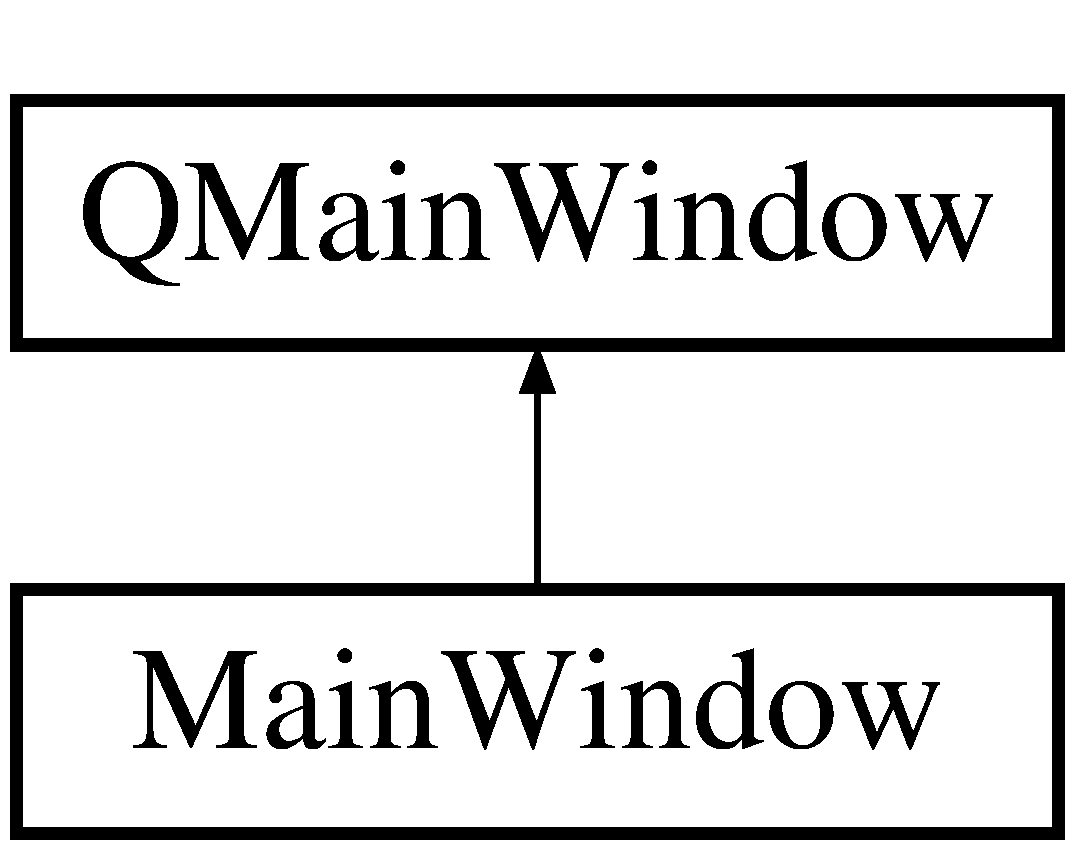
\includegraphics[height=2.000000cm]{class_main_window}
\end{center}
\end{figure}
\subsection*{Public Member Functions}
\begin{DoxyCompactItemize}
\item 
\mbox{\Hypertarget{class_main_window_a8b244be8b7b7db1b08de2a2acb9409db}\label{class_main_window_a8b244be8b7b7db1b08de2a2acb9409db}} 
{\bfseries Main\+Window} (Q\+Widget $\ast$parent=0)
\end{DoxyCompactItemize}


The documentation for this class was generated from the following files\+:\begin{DoxyCompactItemize}
\item 
mainwindow.\+h\item 
mainwindow.\+cpp\end{DoxyCompactItemize}

\hypertarget{class_menu_item}{}\section{Menu\+Item Class Reference}
\label{class_menu_item}\index{Menu\+Item@{Menu\+Item}}


The \hyperlink{class_menu_item}{Menu\+Item} class.  




{\ttfamily \#include $<$menuitem.\+h$>$}

\subsection*{Public Member Functions}
\begin{DoxyCompactItemize}
\item 
\mbox{\Hypertarget{class_menu_item_ace4fef81d61df85c799b17027b83f3ab}\label{class_menu_item_ace4fef81d61df85c799b17027b83f3ab}} 
{\bfseries Menu\+Item} (Q\+String item\+Name, int restaurant\+ID, double price)
\item 
void \hyperlink{class_menu_item_abc651e3a5656b7fbb0e72085b8adab0e}{set\+Item\+Name} (Q\+String item\+Name)
\begin{DoxyCompactList}\small\item\em set\+Item\+Name \end{DoxyCompactList}\item 
void \hyperlink{class_menu_item_a046acac8a4f20c6d3589ac34bb53ea71}{set\+Restaurant\+ID} (int restaurant\+ID)
\begin{DoxyCompactList}\small\item\em set\+Restaurant\+ID \end{DoxyCompactList}\item 
void \hyperlink{class_menu_item_ae2ebb751e94c46e5bbe32dc2f8003919}{set\+Price} (double price)
\begin{DoxyCompactList}\small\item\em set\+Price \end{DoxyCompactList}\item 
Q\+String \hyperlink{class_menu_item_a4d6f0c0ce06292a95521c2f01c360393}{get\+Item\+Name} ()
\begin{DoxyCompactList}\small\item\em get\+Item\+Name \end{DoxyCompactList}\item 
int \hyperlink{class_menu_item_acb28f30d43a514d5f4e9598b5c6f3f60}{get\+Restaurant\+ID} ()
\begin{DoxyCompactList}\small\item\em get\+Restaurant\+ID \end{DoxyCompactList}\item 
double \hyperlink{class_menu_item_a5b9bbfe9c37ff669a5e3b21c171e28a0}{get\+Price} ()
\begin{DoxyCompactList}\small\item\em get\+Price \end{DoxyCompactList}\item 
bool \hyperlink{class_menu_item_a32972e702a424fc12cf96c561dbc5698}{operator==} (\hyperlink{class_menu_item}{Menu\+Item} item\+To\+Compare)
\begin{DoxyCompactList}\small\item\em operator == \end{DoxyCompactList}\end{DoxyCompactItemize}


\subsection{Detailed Description}
The \hyperlink{class_menu_item}{Menu\+Item} class. 

\begin{DoxyAuthor}{Author}
Sean O\textquotesingle{}Hearn Container for menu items that will be stored in a restaurant object 
\end{DoxyAuthor}


\subsection{Member Function Documentation}
\mbox{\Hypertarget{class_menu_item_a4d6f0c0ce06292a95521c2f01c360393}\label{class_menu_item_a4d6f0c0ce06292a95521c2f01c360393}} 
\index{Menu\+Item@{Menu\+Item}!get\+Item\+Name@{get\+Item\+Name}}
\index{get\+Item\+Name@{get\+Item\+Name}!Menu\+Item@{Menu\+Item}}
\subsubsection{\texorpdfstring{get\+Item\+Name()}{getItemName()}}
{\footnotesize\ttfamily Q\+String Menu\+Item\+::get\+Item\+Name (\begin{DoxyParamCaption}{ }\end{DoxyParamCaption})}



get\+Item\+Name 

\begin{DoxyReturn}{Returns}
item\+Name 
\end{DoxyReturn}
\mbox{\Hypertarget{class_menu_item_a5b9bbfe9c37ff669a5e3b21c171e28a0}\label{class_menu_item_a5b9bbfe9c37ff669a5e3b21c171e28a0}} 
\index{Menu\+Item@{Menu\+Item}!get\+Price@{get\+Price}}
\index{get\+Price@{get\+Price}!Menu\+Item@{Menu\+Item}}
\subsubsection{\texorpdfstring{get\+Price()}{getPrice()}}
{\footnotesize\ttfamily double Menu\+Item\+::get\+Price (\begin{DoxyParamCaption}{ }\end{DoxyParamCaption})}



get\+Price 

\begin{DoxyReturn}{Returns}
price 
\end{DoxyReturn}
\mbox{\Hypertarget{class_menu_item_acb28f30d43a514d5f4e9598b5c6f3f60}\label{class_menu_item_acb28f30d43a514d5f4e9598b5c6f3f60}} 
\index{Menu\+Item@{Menu\+Item}!get\+Restaurant\+ID@{get\+Restaurant\+ID}}
\index{get\+Restaurant\+ID@{get\+Restaurant\+ID}!Menu\+Item@{Menu\+Item}}
\subsubsection{\texorpdfstring{get\+Restaurant\+I\+D()}{getRestaurantID()}}
{\footnotesize\ttfamily int Menu\+Item\+::get\+Restaurant\+ID (\begin{DoxyParamCaption}{ }\end{DoxyParamCaption})}



get\+Restaurant\+ID 

\begin{DoxyReturn}{Returns}
restaurant\+ID 
\end{DoxyReturn}
\mbox{\Hypertarget{class_menu_item_a32972e702a424fc12cf96c561dbc5698}\label{class_menu_item_a32972e702a424fc12cf96c561dbc5698}} 
\index{Menu\+Item@{Menu\+Item}!operator==@{operator==}}
\index{operator==@{operator==}!Menu\+Item@{Menu\+Item}}
\subsubsection{\texorpdfstring{operator==()}{operator==()}}
{\footnotesize\ttfamily bool Menu\+Item\+::operator== (\begin{DoxyParamCaption}\item[{\hyperlink{class_menu_item}{Menu\+Item}}]{item\+To\+Compare }\end{DoxyParamCaption})\hspace{0.3cm}{\ttfamily [inline]}}



operator == 


\begin{DoxyParams}{Parameters}
{\em item\+To\+Compare} & \\
\hline
\end{DoxyParams}
\begin{DoxyReturn}{Returns}
bool value 
\end{DoxyReturn}
\mbox{\Hypertarget{class_menu_item_abc651e3a5656b7fbb0e72085b8adab0e}\label{class_menu_item_abc651e3a5656b7fbb0e72085b8adab0e}} 
\index{Menu\+Item@{Menu\+Item}!set\+Item\+Name@{set\+Item\+Name}}
\index{set\+Item\+Name@{set\+Item\+Name}!Menu\+Item@{Menu\+Item}}
\subsubsection{\texorpdfstring{set\+Item\+Name()}{setItemName()}}
{\footnotesize\ttfamily void Menu\+Item\+::set\+Item\+Name (\begin{DoxyParamCaption}\item[{Q\+String}]{item\+Name }\end{DoxyParamCaption})}



set\+Item\+Name 


\begin{DoxyParams}{Parameters}
{\em item\+Name} & \\
\hline
\end{DoxyParams}
\mbox{\Hypertarget{class_menu_item_ae2ebb751e94c46e5bbe32dc2f8003919}\label{class_menu_item_ae2ebb751e94c46e5bbe32dc2f8003919}} 
\index{Menu\+Item@{Menu\+Item}!set\+Price@{set\+Price}}
\index{set\+Price@{set\+Price}!Menu\+Item@{Menu\+Item}}
\subsubsection{\texorpdfstring{set\+Price()}{setPrice()}}
{\footnotesize\ttfamily void Menu\+Item\+::set\+Price (\begin{DoxyParamCaption}\item[{double}]{price }\end{DoxyParamCaption})}



set\+Price 


\begin{DoxyParams}{Parameters}
{\em price} & \\
\hline
\end{DoxyParams}
\mbox{\Hypertarget{class_menu_item_a046acac8a4f20c6d3589ac34bb53ea71}\label{class_menu_item_a046acac8a4f20c6d3589ac34bb53ea71}} 
\index{Menu\+Item@{Menu\+Item}!set\+Restaurant\+ID@{set\+Restaurant\+ID}}
\index{set\+Restaurant\+ID@{set\+Restaurant\+ID}!Menu\+Item@{Menu\+Item}}
\subsubsection{\texorpdfstring{set\+Restaurant\+I\+D()}{setRestaurantID()}}
{\footnotesize\ttfamily void Menu\+Item\+::set\+Restaurant\+ID (\begin{DoxyParamCaption}\item[{int}]{restaurant\+ID }\end{DoxyParamCaption})}



set\+Restaurant\+ID 


\begin{DoxyParams}{Parameters}
{\em restaurant\+ID} & \\
\hline
\end{DoxyParams}


The documentation for this class was generated from the following files\+:\begin{DoxyCompactItemize}
\item 
menuitem.\+h\item 
menuitem.\+cpp\end{DoxyCompactItemize}

\hypertarget{class_restaurant}{}\section{Restaurant Class Reference}
\label{class_restaurant}\index{Restaurant@{Restaurant}}


The \hyperlink{class_restaurant}{Restaurant} class.  




{\ttfamily \#include $<$restaurant.\+h$>$}

\subsection*{Public Member Functions}
\begin{DoxyCompactItemize}
\item 
\mbox{\Hypertarget{class_restaurant_a18bc8aa1ce501a92842a2090e7d378cc}\label{class_restaurant_a18bc8aa1ce501a92842a2090e7d378cc}} 
{\bfseries Restaurant} (Q\+String name, int id, double distance\+From\+Saddleback, int menu\+Size, int total\+Distances)
\item 
void \hyperlink{class_restaurant_aec426da0e4c067525fdd1d233c32a5f3}{set\+Name} (Q\+String name)
\begin{DoxyCompactList}\small\item\em set\+Name \end{DoxyCompactList}\item 
void \hyperlink{class_restaurant_a156dd173f171f1f170191dadb7153b8f}{set\+ID} (int id)
\begin{DoxyCompactList}\small\item\em set\+ID \end{DoxyCompactList}\item 
void \hyperlink{class_restaurant_a12aea2979807bd2132f16f706b634ad4}{set\+Distance\+From\+Saddleback} (double distance\+From\+Saddleback)
\begin{DoxyCompactList}\small\item\em set\+Distance\+From\+Saddleback \end{DoxyCompactList}\item 
void \hyperlink{class_restaurant_aa4a36310566791865760329edb61dfef}{set\+Menu\+Size} (int menu\+Size)
\begin{DoxyCompactList}\small\item\em set\+Menu\+Size \end{DoxyCompactList}\item 
void \hyperlink{class_restaurant_a014e06c350423b40fcfdac1bcbdd6ab1}{set\+Total\+Distances} (int total\+Distances)
\begin{DoxyCompactList}\small\item\em set\+Total\+Distances \end{DoxyCompactList}\item 
void \hyperlink{class_restaurant_a13b2e8a16f44e2fc4304e4b8689e1336}{set\+Visited} (bool visited)
\begin{DoxyCompactList}\small\item\em set\+Visited \end{DoxyCompactList}\item 
\mbox{\Hypertarget{class_restaurant_a47d4e993832e37a98fd4e3f3201b62c4}\label{class_restaurant_a47d4e993832e37a98fd4e3f3201b62c4}} 
Q\+String {\bfseries get\+Name} ()
\item 
int \hyperlink{class_restaurant_a8777e6d48839e275744145f394bde846}{get\+ID} ()
\begin{DoxyCompactList}\small\item\em get\+ID \end{DoxyCompactList}\item 
double \hyperlink{class_restaurant_a328d55dfff742bf89d6b81a01bab35d9}{get\+Distance\+From\+Saddleback} ()
\begin{DoxyCompactList}\small\item\em get\+Distance\+From\+Saddleback \end{DoxyCompactList}\item 
int \hyperlink{class_restaurant_a228a01608b506e6a8bf72b7d6f747a7d}{get\+Menu\+Size} ()
\begin{DoxyCompactList}\small\item\em get\+Menu\+Size \end{DoxyCompactList}\item 
int \hyperlink{class_restaurant_aefc0ab4b34d2ff5cfc5ab0d9463cf224}{get\+Total\+Distances} ()
\begin{DoxyCompactList}\small\item\em get\+Total\+Distances \end{DoxyCompactList}\item 
bool \hyperlink{class_restaurant_a174725e8ae4487dbb649dd9cc017945e}{get\+Visited} ()
\begin{DoxyCompactList}\small\item\em get\+Visited \end{DoxyCompactList}\item 
void \hyperlink{class_restaurant_a35210fa764ffb3ec4c9563c3bb12fd68}{add\+Distance} (\hyperlink{class_distance}{Distance} distance)
\begin{DoxyCompactList}\small\item\em add\+Distance \end{DoxyCompactList}\item 
void \hyperlink{class_restaurant_a5e743b42c3d5277a5c30728e5a6010f0}{add\+Menu\+Item} (\hyperlink{class_menu_item}{Menu\+Item} menu\+Item)
\begin{DoxyCompactList}\small\item\em \hyperlink{classadd_menu_item}{add\+Menu\+Item} \end{DoxyCompactList}\item 
std\+::vector$<$ \hyperlink{class_distance}{Distance} $>$ \hyperlink{class_restaurant_a4b76f9f7171cb961e33bb670c22e91f0}{get\+Distances} ()
\begin{DoxyCompactList}\small\item\em get\+Distances \end{DoxyCompactList}\item 
std\+::vector$<$ \hyperlink{class_menu_item}{Menu\+Item} $>$ \hyperlink{class_restaurant_a67da76f6ae80d9c22c8c697ebbb8a684}{get\+Menu} ()
\begin{DoxyCompactList}\small\item\em get\+Menu \end{DoxyCompactList}\item 
void \hyperlink{class_restaurant_a084b4300b60a5d76cbdcbe01724ba5a6}{set\+Total\+Amount\+Spent} (double amt)
\begin{DoxyCompactList}\small\item\em set\+Total\+Amount\+Spent \end{DoxyCompactList}\item 
double \hyperlink{class_restaurant_a983d7e6327f4f88d9d5aefe4d6beb7c0}{get\+Total\+Amount\+Spent} ()
\begin{DoxyCompactList}\small\item\em get\+Total\+Amount\+Spent \end{DoxyCompactList}\item 
bool \hyperlink{class_restaurant_ac8b5a5436f9e3952f64abc32dc02a82b}{operator==} (\hyperlink{class_restaurant}{Restaurant} restaurant\+To\+Compare)
\begin{DoxyCompactList}\small\item\em operator == \end{DoxyCompactList}\end{DoxyCompactItemize}


\subsection{Detailed Description}
The \hyperlink{class_restaurant}{Restaurant} class. 

\begin{DoxyAuthor}{Author}
Sean O\textquotesingle{}Hearn Container for restaurant objects 
\end{DoxyAuthor}


\subsection{Member Function Documentation}
\mbox{\Hypertarget{class_restaurant_a35210fa764ffb3ec4c9563c3bb12fd68}\label{class_restaurant_a35210fa764ffb3ec4c9563c3bb12fd68}} 
\index{Restaurant@{Restaurant}!add\+Distance@{add\+Distance}}
\index{add\+Distance@{add\+Distance}!Restaurant@{Restaurant}}
\subsubsection{\texorpdfstring{add\+Distance()}{addDistance()}}
{\footnotesize\ttfamily void Restaurant\+::add\+Distance (\begin{DoxyParamCaption}\item[{\hyperlink{class_distance}{Distance}}]{distance }\end{DoxyParamCaption})}



add\+Distance 


\begin{DoxyParams}{Parameters}
{\em distance} & \\
\hline
\end{DoxyParams}
\mbox{\Hypertarget{class_restaurant_a5e743b42c3d5277a5c30728e5a6010f0}\label{class_restaurant_a5e743b42c3d5277a5c30728e5a6010f0}} 
\index{Restaurant@{Restaurant}!add\+Menu\+Item@{add\+Menu\+Item}}
\index{add\+Menu\+Item@{add\+Menu\+Item}!Restaurant@{Restaurant}}
\subsubsection{\texorpdfstring{add\+Menu\+Item()}{addMenuItem()}}
{\footnotesize\ttfamily void Restaurant\+::add\+Menu\+Item (\begin{DoxyParamCaption}\item[{\hyperlink{class_menu_item}{Menu\+Item}}]{menu\+Item }\end{DoxyParamCaption})}



\hyperlink{classadd_menu_item}{add\+Menu\+Item} 


\begin{DoxyParams}{Parameters}
{\em menu\+Item} & \\
\hline
\end{DoxyParams}
\mbox{\Hypertarget{class_restaurant_a328d55dfff742bf89d6b81a01bab35d9}\label{class_restaurant_a328d55dfff742bf89d6b81a01bab35d9}} 
\index{Restaurant@{Restaurant}!get\+Distance\+From\+Saddleback@{get\+Distance\+From\+Saddleback}}
\index{get\+Distance\+From\+Saddleback@{get\+Distance\+From\+Saddleback}!Restaurant@{Restaurant}}
\subsubsection{\texorpdfstring{get\+Distance\+From\+Saddleback()}{getDistanceFromSaddleback()}}
{\footnotesize\ttfamily double Restaurant\+::get\+Distance\+From\+Saddleback (\begin{DoxyParamCaption}{ }\end{DoxyParamCaption})}



get\+Distance\+From\+Saddleback 

\begin{DoxyReturn}{Returns}
distance\+From\+Saddleback 
\end{DoxyReturn}
\mbox{\Hypertarget{class_restaurant_a4b76f9f7171cb961e33bb670c22e91f0}\label{class_restaurant_a4b76f9f7171cb961e33bb670c22e91f0}} 
\index{Restaurant@{Restaurant}!get\+Distances@{get\+Distances}}
\index{get\+Distances@{get\+Distances}!Restaurant@{Restaurant}}
\subsubsection{\texorpdfstring{get\+Distances()}{getDistances()}}
{\footnotesize\ttfamily std\+::vector$<$ \hyperlink{class_distance}{Distance} $>$ Restaurant\+::get\+Distances (\begin{DoxyParamCaption}{ }\end{DoxyParamCaption})}



get\+Distances 

\begin{DoxyReturn}{Returns}
distances 
\end{DoxyReturn}
\mbox{\Hypertarget{class_restaurant_a8777e6d48839e275744145f394bde846}\label{class_restaurant_a8777e6d48839e275744145f394bde846}} 
\index{Restaurant@{Restaurant}!get\+ID@{get\+ID}}
\index{get\+ID@{get\+ID}!Restaurant@{Restaurant}}
\subsubsection{\texorpdfstring{get\+I\+D()}{getID()}}
{\footnotesize\ttfamily int Restaurant\+::get\+ID (\begin{DoxyParamCaption}{ }\end{DoxyParamCaption})}



get\+ID 

\begin{DoxyReturn}{Returns}
ID 
\end{DoxyReturn}
\mbox{\Hypertarget{class_restaurant_a67da76f6ae80d9c22c8c697ebbb8a684}\label{class_restaurant_a67da76f6ae80d9c22c8c697ebbb8a684}} 
\index{Restaurant@{Restaurant}!get\+Menu@{get\+Menu}}
\index{get\+Menu@{get\+Menu}!Restaurant@{Restaurant}}
\subsubsection{\texorpdfstring{get\+Menu()}{getMenu()}}
{\footnotesize\ttfamily std\+::vector$<$ \hyperlink{class_menu_item}{Menu\+Item} $>$ Restaurant\+::get\+Menu (\begin{DoxyParamCaption}{ }\end{DoxyParamCaption})}



get\+Menu 

\begin{DoxyReturn}{Returns}
menu 
\end{DoxyReturn}
\mbox{\Hypertarget{class_restaurant_a228a01608b506e6a8bf72b7d6f747a7d}\label{class_restaurant_a228a01608b506e6a8bf72b7d6f747a7d}} 
\index{Restaurant@{Restaurant}!get\+Menu\+Size@{get\+Menu\+Size}}
\index{get\+Menu\+Size@{get\+Menu\+Size}!Restaurant@{Restaurant}}
\subsubsection{\texorpdfstring{get\+Menu\+Size()}{getMenuSize()}}
{\footnotesize\ttfamily int Restaurant\+::get\+Menu\+Size (\begin{DoxyParamCaption}{ }\end{DoxyParamCaption})}



get\+Menu\+Size 

\begin{DoxyReturn}{Returns}
menu\+Size 
\end{DoxyReturn}
\mbox{\Hypertarget{class_restaurant_a983d7e6327f4f88d9d5aefe4d6beb7c0}\label{class_restaurant_a983d7e6327f4f88d9d5aefe4d6beb7c0}} 
\index{Restaurant@{Restaurant}!get\+Total\+Amount\+Spent@{get\+Total\+Amount\+Spent}}
\index{get\+Total\+Amount\+Spent@{get\+Total\+Amount\+Spent}!Restaurant@{Restaurant}}
\subsubsection{\texorpdfstring{get\+Total\+Amount\+Spent()}{getTotalAmountSpent()}}
{\footnotesize\ttfamily double Restaurant\+::get\+Total\+Amount\+Spent (\begin{DoxyParamCaption}{ }\end{DoxyParamCaption})}



get\+Total\+Amount\+Spent 

\begin{DoxyReturn}{Returns}
total\+Amount\+Spent 
\end{DoxyReturn}
\mbox{\Hypertarget{class_restaurant_aefc0ab4b34d2ff5cfc5ab0d9463cf224}\label{class_restaurant_aefc0ab4b34d2ff5cfc5ab0d9463cf224}} 
\index{Restaurant@{Restaurant}!get\+Total\+Distances@{get\+Total\+Distances}}
\index{get\+Total\+Distances@{get\+Total\+Distances}!Restaurant@{Restaurant}}
\subsubsection{\texorpdfstring{get\+Total\+Distances()}{getTotalDistances()}}
{\footnotesize\ttfamily int Restaurant\+::get\+Total\+Distances (\begin{DoxyParamCaption}{ }\end{DoxyParamCaption})}



get\+Total\+Distances 

\begin{DoxyReturn}{Returns}
total\+Distances 
\end{DoxyReturn}
\mbox{\Hypertarget{class_restaurant_a174725e8ae4487dbb649dd9cc017945e}\label{class_restaurant_a174725e8ae4487dbb649dd9cc017945e}} 
\index{Restaurant@{Restaurant}!get\+Visited@{get\+Visited}}
\index{get\+Visited@{get\+Visited}!Restaurant@{Restaurant}}
\subsubsection{\texorpdfstring{get\+Visited()}{getVisited()}}
{\footnotesize\ttfamily bool Restaurant\+::get\+Visited (\begin{DoxyParamCaption}{ }\end{DoxyParamCaption})\hspace{0.3cm}{\ttfamily [inline]}}



get\+Visited 

\begin{DoxyReturn}{Returns}

\end{DoxyReturn}
\mbox{\Hypertarget{class_restaurant_ac8b5a5436f9e3952f64abc32dc02a82b}\label{class_restaurant_ac8b5a5436f9e3952f64abc32dc02a82b}} 
\index{Restaurant@{Restaurant}!operator==@{operator==}}
\index{operator==@{operator==}!Restaurant@{Restaurant}}
\subsubsection{\texorpdfstring{operator==()}{operator==()}}
{\footnotesize\ttfamily bool Restaurant\+::operator== (\begin{DoxyParamCaption}\item[{\hyperlink{class_restaurant}{Restaurant}}]{restaurant\+To\+Compare }\end{DoxyParamCaption})\hspace{0.3cm}{\ttfamily [inline]}}



operator == 


\begin{DoxyParams}{Parameters}
{\em restaurant\+To\+Compare} & \\
\hline
\end{DoxyParams}
\begin{DoxyReturn}{Returns}
bool value 
\end{DoxyReturn}
\mbox{\Hypertarget{class_restaurant_a12aea2979807bd2132f16f706b634ad4}\label{class_restaurant_a12aea2979807bd2132f16f706b634ad4}} 
\index{Restaurant@{Restaurant}!set\+Distance\+From\+Saddleback@{set\+Distance\+From\+Saddleback}}
\index{set\+Distance\+From\+Saddleback@{set\+Distance\+From\+Saddleback}!Restaurant@{Restaurant}}
\subsubsection{\texorpdfstring{set\+Distance\+From\+Saddleback()}{setDistanceFromSaddleback()}}
{\footnotesize\ttfamily void Restaurant\+::set\+Distance\+From\+Saddleback (\begin{DoxyParamCaption}\item[{double}]{distance\+From\+Saddleback }\end{DoxyParamCaption})}



set\+Distance\+From\+Saddleback 


\begin{DoxyParams}{Parameters}
{\em distance\+From\+Saddleback} & \\
\hline
\end{DoxyParams}
\mbox{\Hypertarget{class_restaurant_a156dd173f171f1f170191dadb7153b8f}\label{class_restaurant_a156dd173f171f1f170191dadb7153b8f}} 
\index{Restaurant@{Restaurant}!set\+ID@{set\+ID}}
\index{set\+ID@{set\+ID}!Restaurant@{Restaurant}}
\subsubsection{\texorpdfstring{set\+I\+D()}{setID()}}
{\footnotesize\ttfamily void Restaurant\+::set\+ID (\begin{DoxyParamCaption}\item[{int}]{id }\end{DoxyParamCaption})}



set\+ID 


\begin{DoxyParams}{Parameters}
{\em id} & \\
\hline
\end{DoxyParams}
\mbox{\Hypertarget{class_restaurant_aa4a36310566791865760329edb61dfef}\label{class_restaurant_aa4a36310566791865760329edb61dfef}} 
\index{Restaurant@{Restaurant}!set\+Menu\+Size@{set\+Menu\+Size}}
\index{set\+Menu\+Size@{set\+Menu\+Size}!Restaurant@{Restaurant}}
\subsubsection{\texorpdfstring{set\+Menu\+Size()}{setMenuSize()}}
{\footnotesize\ttfamily void Restaurant\+::set\+Menu\+Size (\begin{DoxyParamCaption}\item[{int}]{menu\+Size }\end{DoxyParamCaption})}



set\+Menu\+Size 


\begin{DoxyParams}{Parameters}
{\em menu\+Size} & \\
\hline
\end{DoxyParams}
\mbox{\Hypertarget{class_restaurant_aec426da0e4c067525fdd1d233c32a5f3}\label{class_restaurant_aec426da0e4c067525fdd1d233c32a5f3}} 
\index{Restaurant@{Restaurant}!set\+Name@{set\+Name}}
\index{set\+Name@{set\+Name}!Restaurant@{Restaurant}}
\subsubsection{\texorpdfstring{set\+Name()}{setName()}}
{\footnotesize\ttfamily void Restaurant\+::set\+Name (\begin{DoxyParamCaption}\item[{Q\+String}]{name }\end{DoxyParamCaption})}



set\+Name 


\begin{DoxyParams}{Parameters}
{\em name} & \\
\hline
\end{DoxyParams}
\mbox{\Hypertarget{class_restaurant_a084b4300b60a5d76cbdcbe01724ba5a6}\label{class_restaurant_a084b4300b60a5d76cbdcbe01724ba5a6}} 
\index{Restaurant@{Restaurant}!set\+Total\+Amount\+Spent@{set\+Total\+Amount\+Spent}}
\index{set\+Total\+Amount\+Spent@{set\+Total\+Amount\+Spent}!Restaurant@{Restaurant}}
\subsubsection{\texorpdfstring{set\+Total\+Amount\+Spent()}{setTotalAmountSpent()}}
{\footnotesize\ttfamily void Restaurant\+::set\+Total\+Amount\+Spent (\begin{DoxyParamCaption}\item[{double}]{amt }\end{DoxyParamCaption})}



set\+Total\+Amount\+Spent 


\begin{DoxyParams}{Parameters}
{\em amt} & \\
\hline
\end{DoxyParams}
\mbox{\Hypertarget{class_restaurant_a014e06c350423b40fcfdac1bcbdd6ab1}\label{class_restaurant_a014e06c350423b40fcfdac1bcbdd6ab1}} 
\index{Restaurant@{Restaurant}!set\+Total\+Distances@{set\+Total\+Distances}}
\index{set\+Total\+Distances@{set\+Total\+Distances}!Restaurant@{Restaurant}}
\subsubsection{\texorpdfstring{set\+Total\+Distances()}{setTotalDistances()}}
{\footnotesize\ttfamily void Restaurant\+::set\+Total\+Distances (\begin{DoxyParamCaption}\item[{int}]{total\+Distances }\end{DoxyParamCaption})}



set\+Total\+Distances 


\begin{DoxyParams}{Parameters}
{\em total\+Distances} & \\
\hline
\end{DoxyParams}
\mbox{\Hypertarget{class_restaurant_a13b2e8a16f44e2fc4304e4b8689e1336}\label{class_restaurant_a13b2e8a16f44e2fc4304e4b8689e1336}} 
\index{Restaurant@{Restaurant}!set\+Visited@{set\+Visited}}
\index{set\+Visited@{set\+Visited}!Restaurant@{Restaurant}}
\subsubsection{\texorpdfstring{set\+Visited()}{setVisited()}}
{\footnotesize\ttfamily void Restaurant\+::set\+Visited (\begin{DoxyParamCaption}\item[{bool}]{visited }\end{DoxyParamCaption})\hspace{0.3cm}{\ttfamily [inline]}}



set\+Visited 


\begin{DoxyParams}{Parameters}
{\em visited} & \\
\hline
\end{DoxyParams}


The documentation for this class was generated from the following files\+:\begin{DoxyCompactItemize}
\item 
restaurant.\+h\item 
restaurant.\+cpp\end{DoxyCompactItemize}

\hypertarget{class_trip_screen}{}\section{Trip\+Screen Class Reference}
\label{class_trip_screen}\index{Trip\+Screen@{Trip\+Screen}}
Inheritance diagram for Trip\+Screen\+:\begin{figure}[H]
\begin{center}
\leavevmode
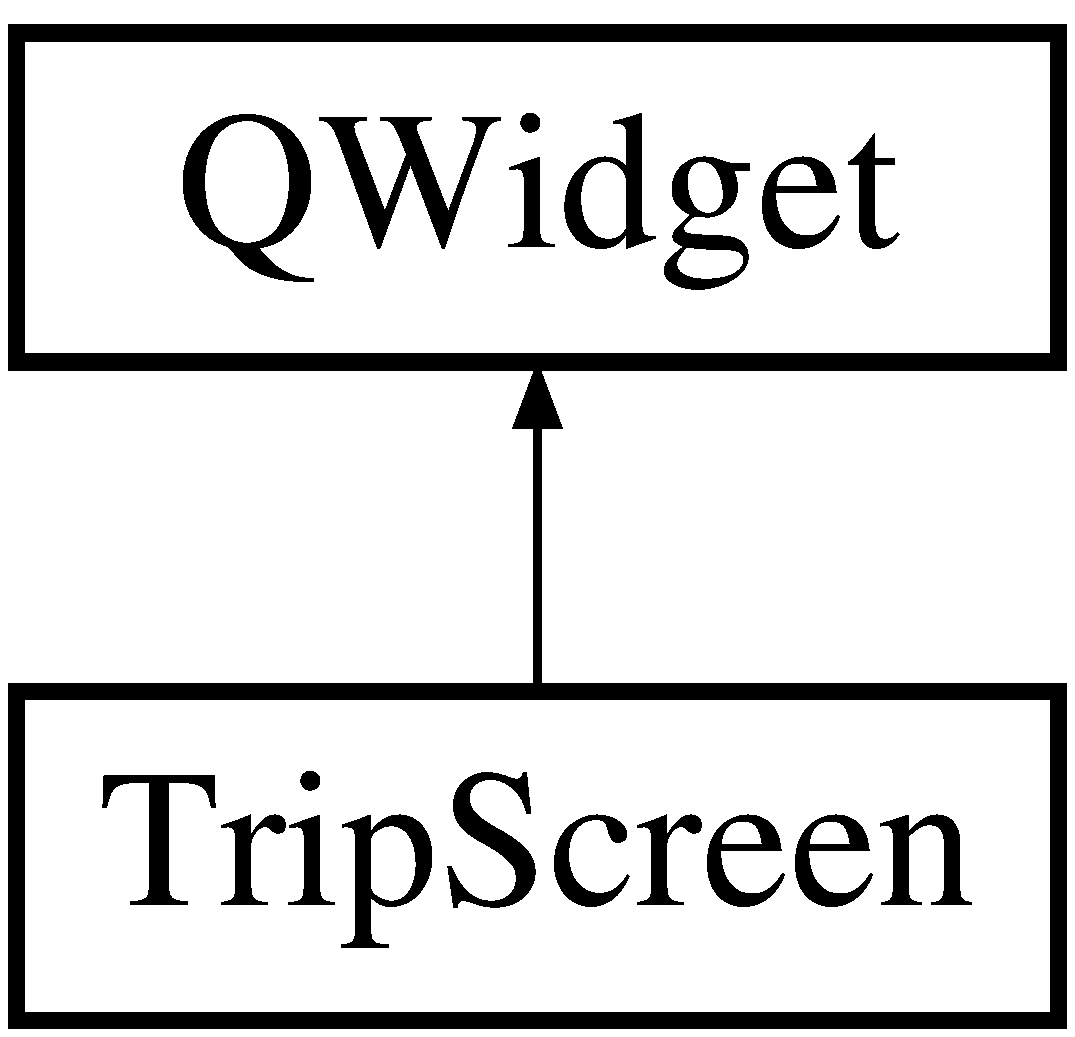
\includegraphics[height=2.000000cm]{class_trip_screen}
\end{center}
\end{figure}
\subsection*{Public Member Functions}
\begin{DoxyCompactItemize}
\item 
\mbox{\Hypertarget{class_trip_screen_a5255c8d2e37c6f7c25de348327ec9a71}\label{class_trip_screen_a5255c8d2e37c6f7c25de348327ec9a71}} 
{\bfseries Trip\+Screen} (Q\+Widget $\ast$parent=0)
\item 
\mbox{\Hypertarget{class_trip_screen_a3eef4ff47f5688995cca879683ec5de3}\label{class_trip_screen_a3eef4ff47f5688995cca879683ec5de3}} 
void {\bfseries set\+Is\+Window\+Open} (bool open)
\item 
\mbox{\Hypertarget{class_trip_screen_a45812d1d598595225c392c6cf953690d}\label{class_trip_screen_a45812d1d598595225c392c6cf953690d}} 
bool {\bfseries get\+Is\+Window\+Open} ()
\item 
\mbox{\Hypertarget{class_trip_screen_a8375220d50f17f1722f225223146302b}\label{class_trip_screen_a8375220d50f17f1722f225223146302b}} 
void {\bfseries add\+Restaurant} (\hyperlink{class_restaurant}{Restaurant} to\+Add)
\item 
\mbox{\Hypertarget{class_trip_screen_aca922b35bd83b51faa6bef7b96f05804}\label{class_trip_screen_aca922b35bd83b51faa6bef7b96f05804}} 
void {\bfseries Trip\+Creator} (\hyperlink{class_restaurant}{Restaurant} current, int num\+Of\+Rest, Q\+Vector$<$ \hyperlink{class_restaurant}{Restaurant} $>$ restaurants, double \&total\+Miles)
\item 
\mbox{\Hypertarget{class_trip_screen_a61b3c5991e10294ea7de956ffcc36261}\label{class_trip_screen_a61b3c5991e10294ea7de956ffcc36261}} 
int {\bfseries Find\+Next\+Restaurant} (\hyperlink{class_restaurant}{Restaurant} current, double \&total\+Miles, std\+::vector$<$ int $>$ I\+Ds)
\item 
\mbox{\Hypertarget{class_trip_screen_a4908a18d119ddda8e05d5492a4244d61}\label{class_trip_screen_a4908a18d119ddda8e05d5492a4244d61}} 
std\+::vector$<$ int $>$ {\bfseries Load\+I\+Ds} (Q\+Vector$<$ \hyperlink{class_restaurant}{Restaurant} $>$ list)
\item 
\mbox{\Hypertarget{class_trip_screen_a40e9a4a42eab6f237a1c3ffaabe70e72}\label{class_trip_screen_a40e9a4a42eab6f237a1c3ffaabe70e72}} 
void {\bfseries push\+Button} ()
\item 
\mbox{\Hypertarget{class_trip_screen_a4bd10ca49117a4c40855ea1c7407c9b8}\label{class_trip_screen_a4bd10ca49117a4c40855ea1c7407c9b8}} 
\hyperlink{class_restaurant}{Restaurant} {\bfseries convert\+I\+D\+To\+Rest} (int ID, Q\+Vector$<$ \hyperlink{class_restaurant}{Restaurant} $>$ list)
\item 
\mbox{\Hypertarget{class_trip_screen_ad37000ffd5921c8c177f42acec2da4ba}\label{class_trip_screen_ad37000ffd5921c8c177f42acec2da4ba}} 
void {\bfseries Print\+Order} ()
\end{DoxyCompactItemize}


The documentation for this class was generated from the following files\+:\begin{DoxyCompactItemize}
\item 
tripscreen.\+h\item 
tripscreen.\+cpp\end{DoxyCompactItemize}

%--- End generated contents ---

% Index
\backmatter
\newpage
\phantomsection
\clearemptydoublepage
\addcontentsline{toc}{chapter}{Index}
\printindex

\end{document}
